\documentclass[a4paper, 12pt]{article}
\usepackage[top=1.8cm, bottom=1.8cm, left=1.5cm, right=1.5cm]{geometry}
\usepackage{float}
\usepackage[utf8]{inputenc}
\usepackage{pgfplots}
\pgfplotsset{width=10cm, compat=1.18}



\begin{document}
	
	\begin{center}
		Universidade Federal do Rio Grande do Norte
		
		Departamento de Engenharia da Computação e Automação  
		
		DCA3703 - Programação Paralela  
		
		\textbf{Tarefa 14: Latência de comunicação usando MPI}  
		
		\textbf{Aluno:} Daniel Bruno Trindade da Silva  
	\end{center}  
	
	\section{Introdução}
	
	\hspace{0.62cm}Este relatório tem como objetivo apresentar os conhecimentos adquiridos durante a realização da Tarefa 15 da disciplina de \textbf{Programação Paralela}. A atividade teve como objetivo mensurar o tempo de comunicação entre os processos usando ferramentas do MPI. Para isso será realizada a implementação e análise de um programa que simulasse a difusão de calor em uma barra 1D. 
	
	\section{Enunciado}
	
	\hspace{0.62cm}Implemente uma simulação da difusão de calor em uma barra 1D, dividida entre dois ou mais processos MPI. Cada processo deve simular um trecho da barra com células extras para troca de bordas com vizinhos. Implemente três versões: uma com \texttt{MPI\_Send/MPI\_Recv}, outra com \texttt{MPI\_Isend/ MPI\_Irecv} e \texttt{MPI\_Wait}, e uma terceira usando \texttt{MPI\_Test} para atualizar os pontos internos enquanto aguarda a comunicação. Compare os tempos de execução e discuta os ganhos com sobreposição de comunicação e computação.
	
	\section{Desenvolvimento}
	\hspace{0.62cm}Para atender aos requisitos da atividade, foram desenvolvidas três versões de um programa em C com MPI para simular a difusão de calor unidimensional. 
	
	Em todas as implementações, a barra 1D de tamanho $N$ é dividida entre os $P$ processos MPI, onde cada processo é responsável por calcular a temperatura de um segmento de $N/P$ células. Para permitir a troca de informações de contorno com os processos vizinhos, cada processo aloca duas células extras (ghost cells), uma no início e outra no fim de seu subdomínio local. A inicialização da barra atribui um valor de temperatura elevado a uma célula central da barra global e zero às demais. As condições de contorno globais da barra são fixas em 0.0. O tempo de execução de cada simulação é medido utilizando \texttt{MPI\_Wtime()} e o tempo máximo entre todos os processos é obtido com \texttt{MPI\_Reduce}.
	
	As três versões implementadas diferem na forma como a comunicação das células de borda é realizada da seguinte forma:
	
	\begin{itemize}
		\item \textbf{Versão 1:} - Nesta implementação, a troca de dados das células de borda é realizada utilizando as funções bloqueantes \texttt{MPI\_Send} e \texttt{MPI\_Recv}. A natureza bloqueante dessas chamadas implica que um processo pode ficar ocioso enquanto espera a conclusão de uma operação de envio ou recebimento.
		
		\item \textbf{Versão 2:} - A segunda implementação utiliza as versões não bloqueantes das chamadas de comunicação, \texttt{MPI\_Isend} e \texttt{MPI\_Irecv}, para a troca das células de borda. Após iniciar todas as operações de comunicação necessárias, a função \texttt{MPI\_Waitall} é chamada. Esta função bloqueia o processo até que todas as comunicações não bloqueantes (tanto envios quanto recebimentos) especificadas sejam concluídas. Somente após o retorno de \texttt{MPI\_Waitall}, o cálculo da nova temperatura para todas as células locais é efetuado. Nesta abordagem, embora as operações sejam não bloqueantes, a computação dos pontos da malha só ocorre após a finalização de toda a comunicação.
		
		\item \textbf{Versão 3 (mpi\_test.c):} - Esta terceira versão também emprega chamadas de comunicação não bloqueantes, \texttt{MPI\_Isend} e \texttt{MPI\_Irecv}, para a troca de dados das células de borda. No entanto, adota uma estratégia para tentar sobrepor o cálculo com a comunicação. Após iniciar as operações de envio e recebimento não bloqueantes, o programa prossegue para calcular os valores dos pontos internos do domínio local (aqueles que não são imediatamente adjacentes às células fantasmas), que não dependem dos dados das células fantasmas que estão sendo trocadas naquele momento. Em seguida, utiliza a função \texttt{MPI\_Test} em laços dedicados para verificar ativamente a conclusão das operações de recebimento (\texttt{MPI\_Irecv}) das células de borda. Uma vez que o recebimento de dados de uma borda específica é confirmado por \texttt{MPI\_Test} (indicando que a célula fantasma correspondente foi preenchida), o cálculo para o ponto da malha adjacente a essa borda é realizado. Finalmente, a função \texttt{MPI\_Wait} é chamada para cada operação de envio (\texttt{MPI\_Isend}) para garantir que estas também tenham sido concluídas. Esta abordagem visa maximizar a utilização da CPU, permitindo que os cálculos dos pontos internos ocorram enquanto as comunicações das bordas estão em andamento, e processando os pontos de borda assim que seus dados necessários se tornam disponíveis, antes de garantir a finalização dos envios.
		
	\end{itemize}
	
	\section{Resultados}
	
	\begin{center}
		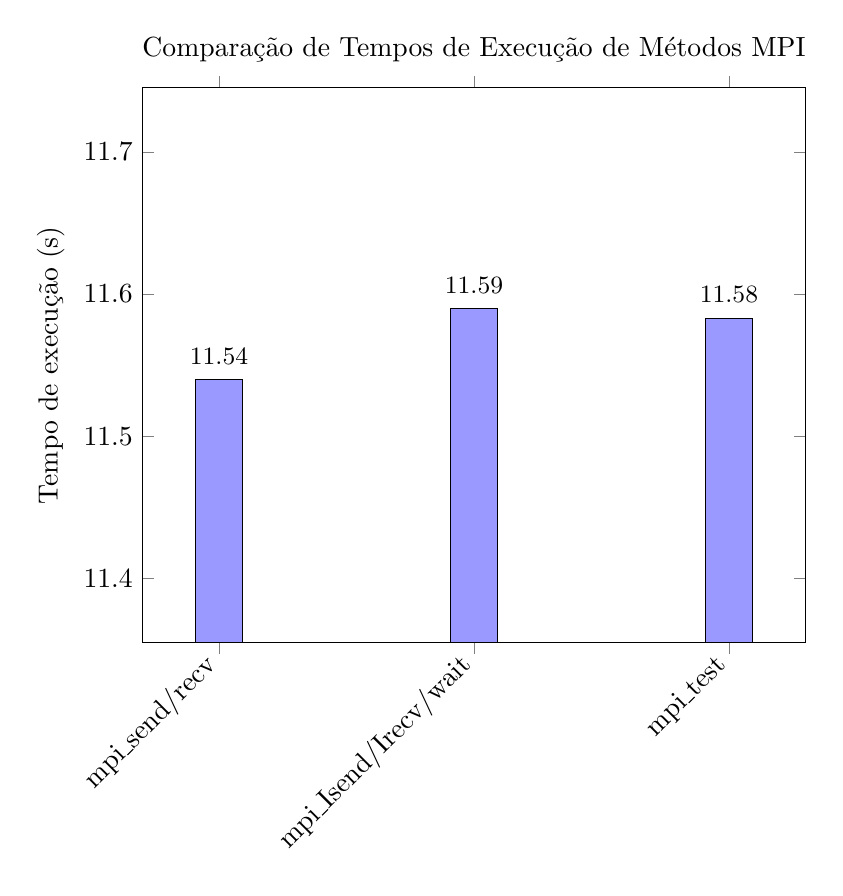
\begin{tikzpicture}
			\begin{axis}[
				title={Comparação de Tempos de Execução de Métodos MPI},
				ybar,
				bar width=0.6cm,
				enlargelimits=0.15,
				legend style={at={(0.5,-0.25)},
					anchor=north,
					legend columns=-1},
				ylabel={Tempo de execução (s)},
				symbolic x coords={mpi\_send/recv, mpi\_Isend/Irecv/wait, mpi\_test},
				xtick=data,
				nodes near coords,
				nodes near coords style={font=\small, yshift=2pt},
				ymin=11.4,  % Valor mínimo do eixo Y
				ymax=11.7,   % Valor máximo do eixo Y
				ytick={11.4,11.5,11.6,11.7},
				xticklabel style={rotate=45, anchor=east},
				point meta=y,  % Mostra valores exatos
				]
				
				\addplot[fill=blue!40] coordinates {
					(mpi\_send/recv, 11.539983)
					(mpi\_Isend/Irecv/wait, 11.589845)
					(mpi\_test, 11.582980)
				};
				
			\end{axis}
		\end{tikzpicture}
	\end{center}
	
\end{document}
